\section{Ten-Solid Equations of State}
\label{sec:solids}

\subsection{Structures and common fit windows}
\label{sec:solid-structures}

The selected solids are AlN, AlP, BN, BP, C, LiCl, MgO, MgS, Si, and SiC from the Goldzak set.\cite{Goldzak2022Solids} All use conventional cubic eight-atom cells. Ten initial volumes are evenly spaced from 0.90 to 1.10 times the static-lattice experimental volume. The common fit window contains the first nine volumes for AlN and AlP, ending at 1.0777778, and all ten for the other solids. The 40 method--solid comparisons derive from 36 independent curves and 352 unique energies: the AE curves for BN and C are shared by both mixed protocols. Third-order Birch--Murnaghan fits give the equilibrium lattice constant and elastic response under isotropic compression.

The comparison uses the ten solids for which consistent EOS data were available in every representation. LiF and LiH are not included. The selection is identical across protocols and was not based on the magnitude of the reference error.

\subsection{Computational details and fit stability}
\label{sec:solid-settings}

All selected points use 800/60~Ry cutoffs, 150 radial points, the 770-point Lebedev rule, and the small extended one-centre basis. All are neutral, spin-restricted calculations with UZH 2026.2 basis and potential definitions.\cite{Mirhosseini2026UZH} GAPW-AE uses TZVPP-MOLOPT-PBE-ae orbital bases and explicit core electrons for every element. GAPW-XC/GTH uses TZV2P-MOLOPT-PBE-GTH bases and the corresponding element-specific GTH-PBE potentials. In the mixed protocols, Li, B, C, N, and O retain the AE TZVPP basis, while Mg, Al, Si, P, S, and Cl use the GTH TZV2P basis. The AE one-centre reconstruction is retained in both mixed protocols. Their direct/one-centre distinction concerns the GTH fields. Every reported energy includes D3(BJ). Diagonalization and OT use residual thresholds of $5\times10^{-6}$ and $5\times10^{-7}$, respectively. Exact inputs specify the remaining dispersion and integration conventions.

The actual Gamma-centred meshes are listed in Table~\ref{tab:actual-k-meshes}. The mesh is identical across representations at each volume but can change with volume within an EOS. Consequently, a smooth fit is not by itself evidence of k-point convergence. The selected full/reduced-mesh checks in the preceding section constrain symmetry reduction for their tested cases, not all possible geometries and restarts.

Every full-window minimum is bracketed. The largest fit RMS residual is 0.674~meV per atom. Omitting one endpoint changes the fitted lattice constant by at most 0.002444~\AA{} (mixed-direct MgS, smallest-volume point omitted) and the bulk modulus by at most 9.997~GPa (GAPW-XC AlN, largest-volume point omitted). The smallest-volume point is essential to bracketing the LiCl minimum. These tests assess fit-window sensitivity. They do not measure basis or quadrature errors and are not transferable error bars for other curves.

\subsection{Basis sensitivity of structural observables}
\label{sec:solid-basis}

The ten independent AE curves contain 98 accepted TZVPP energy points. Paired five-volume QZVPP controls are available for Si, diamond, and MgO. Structural basis convergence must be assessed over volume, separately from SCF convergence and fit stability. For a basis change,
\begin{equation}
 \delta E(V)=E_{\mathrm{QZVPP}}(V)-E_{\mathrm{TZVPP}}(V),
\end{equation}
a constant $\delta E$ changes only the energy origin. Its volume dependence can instead alter the equilibrium volume, curvature, and higher derivatives that determine the elastic response. An accurate fit to a finite-basis curve therefore does not establish basis-converged lattice constants or bulk moduli.

For each solid, we compare the same five volumes, numbered 1, 3, 5, 7, and 9 in the original ten-point series. Geometry, full k-point mesh, core treatment, cutoffs, and quadrature are unchanged at each paired volume. The QZVPP calculations use full point-group reduction, through spglib for Si and diamond and the native K290 backend for MgO, and diagonalization with an SCF threshold of $5\times10^{-6}$. Same-basis checks at volume 5 reproduce the archived TZVPP energies to $1.75\times10^{-7}$~hartree for Si and $6.05\times10^{-9}$~hartree for diamond. The corresponding MgO check at volume 3 differs by $2.56\times10^{-6}$~hartree. These small differences separate the basis effect from changes in the executable and symmetry path.

\begin{table}[htbp]
\centering\small
\caption{Matched five-volume AE basis tests. Lattice constants are in \AA{} and bulk moduli in GPa. Both bases are fitted on the same five volumes. Experimental static-lattice references are from Ref.~\citenum{Goldzak2022Solids}. These three QZVPP controls do not replace the uniform ten-solid TZVPP comparison.}
\label{tab:solid-basis}
\begin{tabular}{llrr}
\toprule
Solid & Basis/reference & $a_0$ & $B_0$\\
\midrule
Si & TZVPP & 5.3747 & 100.36\\
Si & QZVPP & 5.3551 & 106.06\\
Si & Experiment & 5.4210 & 100.30\\
C & TZVPP & 3.5292 & 491.16\\
C & QZVPP & 3.5365 & 475.81\\
C & Experiment & 3.5530 & 453.30\\
MgO & TZVPP & 4.0935 & 198.84\\
MgO & QZVPP & 4.0904 & 197.45\\
MgO & Experiment & 4.1890 & 173.00\\
\bottomrule
\end{tabular}
\end{table}


The response is material dependent (Table~\ref{tab:solid-basis}). For diamond, QZVPP increases $a_0$ by 0.00735~\AA{} and lowers $B_0$ by 15.35~GPa, improving both relative to experiment. For Si, $a_0$ decreases by 0.01950~\AA{} and $B_0$ increases by 5.70~GPa, worsening both errors. MgO changes much less, with shifts of $-0.00307$~\AA{} and $-1.39$~GPa. Its lattice constant remains substantially shorter than experiment, while its bulk modulus improves slightly but remains too large. Across the sampled volumes, the span of $\delta E(V)$ is 18.64, 24.00, and 2.19~meV per atom for diamond, Si, and MgO, respectively. These nonconstant shifts explain why the basis changes affect the fitted structure as well as the absolute energy.

All three five-point minima are bracketed, and the fit RMS residuals remain below 0.19~meV per atom. Omitting either endpoint from a QZVPP fit changes $a_0$ by at most 0.000168~\AA{} for diamond and 0.00165~\AA{} for Si. The corresponding maximum changes in $B_0$ are 5.12 and 8.25~GPa. For MgO, omitting the largest-volume point changes $a_0$ by only 0.000066~\AA{} and $B_0$ by 1.36~GPa. Its smallest-volume point is required to bracket the minimum and is retained in the reported fit. These are fit-window sensitivity measures, not uncertainty estimates. The pressure derivative is more sensitive to these sparse windows and is not used to infer an improved QZVPP prediction. The same-five-volume TZVPP fits reproduce the original ten-volume values within 0.00061~\AA{} and 0.20~GPa, so changing the fit population alone does not account for the basis shifts.

For Si, five additional QZVPP calculations at volumes 2, 4, 6, 8, and 10 complete the original ten-volume series; the five existing QZVPP energies and all TZVPP energies are reused. The added points retain the matched geometry, $4\times4\times4$ mesh, full spglib reduction to ten irreducible points, and the numerical settings above. Table~\ref{tab:si-eos-extension} compares both bases on identical fit windows. The full ten-point fits give $a_0=5.37404$ and 5.35467~\AA{} and $B_0=100.56$ and 106.89~GPa for TZVPP and QZVPP, respectively. The QZVPP shifts of $-0.01938$~\AA{} and $+6.33$~GPa confirm the increased contraction and stiffness relative to the static-lattice reference, 5.421~\AA{} and 100.3~GPa. Fit RMS residuals are 0.350 and 0.403~meV per atom.

Omitting the smallest, largest, or both endpoint volumes leaves every minimum bracketed and preserves the direction of both basis shifts. Across these windows and the full ten-point QZVPP fit, $a_0$ spans 5.35467--5.35589~\AA{}, whereas $B_0$ spans 106.04--112.69~GPa. Thus the additional sampling supports the structural trend but does not remove curvature sensitivity to the chosen fit window. These spans are not statistical uncertainty estimates, and $B'_0$ remains exploratory. Only Si has been extended to ten QZVPP volumes; diamond and MgO retain their five-volume controls.

\begin{table}[htbp]
\centering\small
\caption{Matched Si EOS fits with different sampling and fit windows. Lattice constants are in \AA{}, bulk moduli in GPa, and fit RMS residuals in meV per atom. All minima are bracketed. Five new QZVPP points complete the ten-volume curve; the original five QZVPP points and all TZVPP energies are reused. The uniform ten-solid statistics are unchanged.}
\label{tab:si-eos-extension}
\begin{tabular}{lcrrrr}
\toprule
Window & Basis & $N$ & $a_0$ & $B_0$ & RMS\\
\midrule
Original five & TZVPP & 5 & 5.37465 & 100.36 & 0.153\\
Original five & QZVPP & 5 & 5.35515 & 106.06 & 0.181\\
All ten & TZVPP & 10 & 5.37404 & 100.56 & 0.350\\
All ten & QZVPP & 10 & 5.35467 & 106.89 & 0.403\\
Omit smallest & TZVPP & 9 & 5.37395 & 104.44 & 0.173\\
Omit smallest & QZVPP & 9 & 5.35548 & 112.69 & 0.174\\
Omit largest & TZVPP & 9 & 5.37510 & 100.55 & 0.244\\
Omit largest & QZVPP & 9 & 5.35573 & 106.04 & 0.298\\
Omit both endpoints & TZVPP & 8 & 5.37458 & 103.53 & 0.098\\
Omit both endpoints & QZVPP & 8 & 5.35589 & 111.13 & 0.101\\
\bottomrule
\end{tabular}
\end{table}


The paired molecular-crystal and ice tests identify substantial basis contributions to crystal--molecule energy differences. Their magnitudes cannot be transferred directly to structural observables, which contain no gas-phase reference. The Si, diamond, and MgO controls likewise do not establish basis convergence for all ten solids. The uniform ten-solid comparison below therefore retains its original TZVPP AE protocol. The shared BN and C curves are counted once and do not constitute independent basis checks.

\subsection{Representation and material trends}
\label{sec:solid-trends}

All native lattice constants are below the static-lattice experimental reference. LiCl contracts most, by approximately 0.154--0.164~\AA{}, while C and BN contract by about 0.015--0.026~\AA{}. MgS is also strongly contracted. The common sign spans diamond, zincblende, and rocksalt structures rather than a single bonding class.

GAPW-XC and AE differ on average by 0.01893~\AA{} in $a_0$ and 10.55~GPa in $B_0$, but this comparison changes basis and core treatment as well as density representation. At fixed mixed-core Hamiltonian, the one-centre correction changes $a_0$ by 0.000135~\AA{} on average and at most 0.000542~\AA{} (AlP). The corresponding changes in $B_0$ average 1.11~GPa and reach 5.75~GPa (MgO). Excluding the two shared AE curves gives mean changes of 0.000169~\AA{} and 1.39~GPa over eight independent pairs. The main contraction trend is therefore insensitive to this representation choice.

Curvature errors are less uniform. GAPW-XC underestimates the Si bulk modulus, 92.76 versus 100.3~GPa, despite a contracted lattice, whereas AE gives 100.56~GPa. For C, GAPW-XC is closer to the reference modulus than AE. A shorter equilibrium lattice does not necessarily imply a larger bulk modulus, and AE does not improve every property of every material. Neither $a_0$ nor $B_0$ determines a cohesive energy without atomic references.

\subsection{Matched literature comparisons}
\label{sec:solid-literature}

All methods are compared against the same primary static-lattice experimental values from Goldzak \emph{et al.}\cite{Goldzak2022Solids} Their Hartree--Fock (HF), second-order M{\o}ller--Plesset perturbation theory (MP2), spin-component-scaled MP2 (SCS-MP2), and scaled opposite-spin MP2 (SOS-MP2) results cover all ten selected solids. Zhang \emph{et al.}\cite{Zhang2018Solids} supply local-density approximation (LDA), PBE, PBEsol, M06-L, SCAN, and HSE06 values for nine, excluding AlN. We use their uncorrected static electronic values, not predictions with zero-point corrections. Their SCAN calculations were non-self-consistent on PBE densities. Schimka \emph{et al.}\cite{Schimka2011HSEsol} provide PBE, PBEsol, HSE06, and HSEsol lattice constants for nine, excluding MgS. No missing bulk modulus is inferred. Self-consistent Tao--Mo results\cite{Mo2017Solids} cover eight, excluding AlN and BN, and are rescored against the same Goldzak reference.

Our periodic GFN manuscript\cite{Alizadeh2026PeriodicGFN2} supplies GFN1-xTB and GFN2-xTB lattice constants for nine shared solids, but no bulk moduli in the curated comparison table. Its ten-material set excludes MgO and LiH, whereas the present set excludes LiF and LiH. The two ten-material selections must therefore not be treated as identical.

SCS-MP2 and SOS-MP2 give matched ten-solid lattice MAEs of 0.0125 and 0.0149~\AA{}, and bulk-modulus MAEs of 4.10 and 3.88~GPa. The native ranges are 0.0728--0.0844~\AA{} and 16.61--21.77~GPa. Established semilocal and screened-hybrid methods also have smaller lattice errors on the corresponding intersections. These results identify a limitation of the present structural predictions. The comparisons do not uniquely separate functional and numerical contributions.

Alternative experimental moduli listed by Goldzak \emph{et al.} for BN, BP, and MgO are 410.2, 168.0, and 169.8~GPa, instead of the primary 388.5, 176.5, and 173.0~GPa. Simultaneously replacing all three lowers each native ten-solid modulus MAE by 1.00~GPa and leaves the qualitative conclusion intact. Broader 44-solid statistics, such as those of Tran \emph{et al.},\cite{Tran2016Solids} are not relabelled as matched ten-solid errors.

\begin{table*}[t]
\centering
\small
\caption{Selected $a_0$ values (\AA{}). Experimental references follow Ref.~\citenum{Goldzak2022Solids}. BN and C reuse the AE curve for HD and HOC. These entries are not independent calculations.}
\label{tab:selected-a0_A}
\begin{tabular}{lrrrrr}
\toprule
Solid & Experiment & GX & AE & HD & HOC \\
\midrule
AlN & 4.3680 & 4.2811 & 4.3025 & 4.2747 & 4.2746 \\
AlP & 5.4480 & 5.3622 & 5.3781 & 5.3616 & 5.3621 \\
BN & 3.5930 & 3.5777 & 3.5675 & 3.5675 & 3.5675 \\
BP & 4.5250 & 4.4439 & 4.4696 & 4.4527 & 4.4527 \\
C & 3.5530 & 3.5345 & 3.5292 & 3.5292 & 3.5292 \\
LiCl & 5.0720 & 4.9081 & 4.9155 & 4.9178 & 4.9179 \\
MgO & 4.1890 & 4.1059 & 4.0935 & 4.0923 & 4.0919 \\
MgS & 5.1880 & 5.0689 & 5.0536 & 5.0700 & 5.0697 \\
Si & 5.4210 & 5.3386 & 5.3740 & 5.3383 & 5.3383 \\
SiC & 4.3470 & 4.2517 & 4.2920 & 4.2556 & 4.2556 \\
\bottomrule
\end{tabular}
\end{table*}

\begin{table*}[t]
\centering
\small
\caption{Selected $B_0$ values (GPa). Experimental references follow Ref.~\citenum{Goldzak2022Solids}. BN and C reuse the AE curve for HD and HOC. These entries are not independent calculations.}
\label{tab:selected-B0_GPa}
\begin{tabular}{lrrrrr}
\toprule
Solid & Experiment & GX & AE & HD & HOC \\
\midrule
AlN & 206.00 & 239.07 & 225.89 & 240.42 & 240.40 \\
AlP & 87.00 & 94.34 & 101.35 & 96.36 & 93.12 \\
BN & 388.50 & 423.39 & 420.87 & 420.87 & 420.87 \\
BP & 176.50 & 187.93 & 183.64 & 185.86 & 185.86 \\
C & 453.30 & 457.33 & 491.35 & 491.35 & 491.35 \\
LiCl & 37.30 & 47.98 & 46.37 & 47.13 & 47.16 \\
MgO & 173.00 & 188.28 & 198.71 & 213.13 & 207.37 \\
MgS & 81.00 & 87.90 & 90.27 & 84.17 & 86.22 \\
Si & 100.30 & 92.76 & 100.56 & 94.13 & 94.13 \\
SiC & 228.90 & 263.89 & 241.68 & 263.73 & 263.71 \\
\bottomrule
\end{tabular}
\end{table*}

\begin{table*}[t]
\centering
\small
\caption{EOS fit diagnostics, part 1. All full-window minima are bracketed. RMS residuals are in meV per atom.}
\label{tab:eos-fit-1}
\begin{tabular}{lrrrr}
\toprule
Method & Solid & $N_V$ & $B'_0$ & RMS \\
\midrule
AE & AlN & 9 & 3.707 & 0.0418 \\
AE & AlP & 9 & 4.179 & 0.0880 \\
AE & BN & 10 & 3.772 & 0.1250 \\
AE & BP & 10 & 3.701 & 0.0311 \\
AE & C & 10 & 3.756 & 0.0542 \\
AE & LiCl & 10 & 4.029 & 0.0205 \\
AE & MgO & 10 & 4.092 & 0.0190 \\
AE & MgS & 10 & 3.682 & 0.0117 \\
AE & Si & 10 & 4.544 & 0.3496 \\
AE & SiC & 10 & 3.854 & 0.0449 \\
GX & AlN & 9 & 2.802 & 0.6739 \\
GX & AlP & 9 & 3.959 & 0.1431 \\
GX & BN & 10 & 3.713 & 0.1306 \\
GX & BP & 10 & 4.081 & 0.0723 \\
GX & C & 10 & 3.611 & 0.1734 \\
GX & LiCl & 10 & 4.027 & 0.0435 \\
GX & MgO & 10 & 3.864 & 0.2921 \\
GX & MgS & 10 & 4.349 & 0.1597 \\
\bottomrule
\end{tabular}
\end{table*}

\begin{table*}[t]
\centering
\small
\caption{EOS fit diagnostics, part 2. All full-window minima are bracketed. RMS residuals are in meV per atom.}
\label{tab:eos-fit-2}
\begin{tabular}{lrrrr}
\toprule
Method & Solid & $N_V$ & $B'_0$ & RMS \\
\midrule
GX & Si & 10 & 5.096 & 0.5702 \\
GX & SiC & 10 & 4.107 & 0.1309 \\
HD & AlN & 9 & 3.339 & 0.3028 \\
HD & AlP & 9 & 4.778 & 0.3362 \\
HD & BP & 10 & 3.918 & 0.0532 \\
HD & LiCl & 10 & 3.905 & 0.0330 \\
HD & MgO & 10 & 4.208 & 0.3562 \\
HD & MgS & 10 & 3.167 & 0.2585 \\
HD & Si & 10 & 5.257 & 0.3634 \\
HD & SiC & 10 & 4.168 & 0.0561 \\
HOC & AlN & 9 & 3.338 & 0.3027 \\
HOC & AlP & 9 & 3.787 & 0.2878 \\
HOC & BP & 10 & 3.918 & 0.0532 \\
HOC & LiCl & 10 & 3.915 & 0.0328 \\
HOC & MgO & 10 & 4.181 & 0.0393 \\
HOC & MgS & 10 & 3.865 & 0.0993 \\
HOC & Si & 10 & 5.257 & 0.3634 \\
HOC & SiC & 10 & 4.167 & 0.0557 \\
\bottomrule
\end{tabular}
\end{table*}

\begin{table*}[t]
\centering
\small
\caption{Matched comparison with Ref.~\citenum{Goldzak2022Solids}: ten-solid set. Every row uses the identical intersection and the Goldzak static-lattice experimental reference. MAE($a_0$) is in \AA{} and MAE($B_0$) in GPa. A dash denotes unavailable data, not zero error. Native rows retain the numerical qualifications discussed in the text.}
\label{tab:literature-Goldzak2022}
\begin{tabular}{lrrr}
\toprule
Method & $N$ & MAE($a_0$) & MAE($B_0$) \\
\midrule
GX & 10 & 0.0831 & 16.61 \\
AE & 10 & 0.0728 & 16.89 \\
HD & 10 & 0.0844 & 21.77 \\
HOC & 10 & 0.0844 & 21.07 \\
HF & 10 & 0.0563 & 15.23 \\
MP2 & 10 & 0.0201 & 5.71 \\
SCS-MP2 & 10 & 0.0125 & 4.10 \\
SOS-MP2 & 10 & 0.0149 & 3.88 \\
\bottomrule
\end{tabular}
\end{table*}

\begin{table*}[t]
\centering
\small
\caption{Matched comparison with Ref.~\citenum{Zhang2018Solids}: nine solids, excluding AlN. Every row uses the identical intersection and the Goldzak static-lattice experimental reference. MAE($a_0$) is in \AA{} and MAE($B_0$) in GPa. A dash denotes unavailable data, not zero error. Native rows retain the numerical qualifications discussed in the text.}
\label{tab:literature-Zhang2018}
\begin{tabular}{lrrr}
\toprule
Method & $N$ & MAE($a_0$) & MAE($B_0$) \\
\midrule
GX & 9 & 0.0827 & 14.78 \\
AE & 9 & 0.0737 & 16.56 \\
HD & 9 & 0.0834 & 20.36 \\
HOC & 9 & 0.0835 & 19.59 \\
LDA & 9 & 0.0324 & 4.66 \\
PBE & 9 & 0.0451 & 12.96 \\
PBEsol & 9 & 0.0113 & 4.72 \\
M06-L & 9 & 0.0128 & 3.46 \\
SCAN & 9 & 0.0123 & 3.08 \\
HSE06 & 9 & 0.0170 & 5.86 \\
\bottomrule
\end{tabular}
\end{table*}

\begin{table*}[t]
\centering
\small
\caption{Matched comparison with Ref.~\citenum{Schimka2011HSEsol}: nine solids, excluding MgS. Every row uses the identical intersection and the Goldzak static-lattice experimental reference. MAE($a_0$) is in \AA{} and MAE($B_0$) in GPa. A dash denotes unavailable data, not zero error. Native rows retain the numerical qualifications discussed in the text.}
\label{tab:literature-Schimka2011}
\begin{tabular}{lrrr}
\toprule
Method & $N$ & MAE($a_0$) & MAE($B_0$) \\
\midrule
GX & 9 & 0.0791 & -- \\
AE & 9 & 0.0660 & -- \\
HD & 9 & 0.0807 & -- \\
HOC & 9 & 0.0807 & -- \\
PBE & 9 & 0.0438 & -- \\
PBEsol & 9 & 0.0136 & -- \\
HSE06 & 9 & 0.0132 & -- \\
HSEsol & 9 & 0.0117 & -- \\
\bottomrule
\end{tabular}
\end{table*}

\begin{table*}[t]
\centering
\small
\caption{Matched comparison with Ref.~\citenum{Mo2017Solids}: eight solids, excluding AlN and BN. Every row uses the identical intersection and the Goldzak static-lattice experimental reference. MAE($a_0$) is in \AA{} and MAE($B_0$) in GPa. A dash denotes unavailable data, not zero error. Native rows retain the numerical qualifications discussed in the text.}
\label{tab:literature-Mo2017}
\begin{tabular}{lrrr}
\toprule
Method & $N$ & MAE($a_0$) & MAE($B_0$) \\
\midrule
GX & 8 & 0.0911 & 12.27 \\
AE & 8 & 0.0797 & 14.58 \\
HD & 8 & 0.0907 & 18.86 \\
HOC & 8 & 0.0907 & 18.00 \\
Tao-Mo & 8 & 0.0194 & 4.26 \\
\bottomrule
\end{tabular}
\end{table*}

\begin{table*}[t]
\centering
\small
\caption{Matched comparison with Ref.~\citenum{Alizadeh2026PeriodicGFN2}: nine solids, excluding MgO. Every row uses the identical intersection and the Goldzak static-lattice experimental reference. MAE($a_0$) is in \AA{} and MAE($B_0$) in GPa. A dash denotes unavailable data, not zero error. Native rows retain the numerical qualifications discussed in the text.}
\label{tab:literature-PeriodicGFN2Manuscript}
\begin{tabular}{lrrr}
\toprule
Method & $N$ & MAE($a_0$) & MAE($B_0$) \\
\midrule
GX & 9 & 0.0831 & -- \\
AE & 9 & 0.0703 & -- \\
HD & 9 & 0.0831 & -- \\
HOC & 9 & 0.0830 & -- \\
GFN1-xTB & 9 & 0.1360 & -- \\
GFN2-xTB & 9 & 0.0659 & -- \\
\bottomrule
\end{tabular}
\end{table*}

\begin{table*}[t]
\centering
\small
\caption{Actual Gamma-centered k meshes by volume index. Indices 01--10 refer to the original evenly spaced volume ratios 0.90--1.10. Each selected volume uses the same mesh in all representations, but the mesh can change along an EOS.}
\label{tab:actual-k-meshes}
\begin{tabular}{lr}
\toprule
Solid & Mesh and volume indices \\
\midrule
AlN & $5^3$: 01,02,03,04,05,06,07,08,09 \\
AlP & $4^3$: 01,02,03,04,05,06,07,08,09 \\
BN & $6^3$: 02,03,04,05,06,07,08,09,10; $7^3$: 01 \\
BP & $5^3$: 01,02,03,04,05,06,07,08,09,10 \\
C & $6^3$: 04,05,06,07,08,09,10; $7^3$: 01,02,03 \\
LiCl & $5^3$: 01,02,03,04,05,06,07,08,09,10 \\
MgO & $5^3$: 06,07,08,09,10; $6^3$: 01,02,03,04,05 \\
MgS & $4^3$: 07,08,09,10; $5^3$: 01,02,03,04,05,06 \\
Si & $4^3$: 02,03,04,05,06,07,08,09,10; $5^3$: 01 \\
SiC & $5^3$: 01,02,03,04,05,06,07,08,09,10 \\
\bottomrule
\end{tabular}
\end{table*}

\begin{figure}[htbp]
\centering
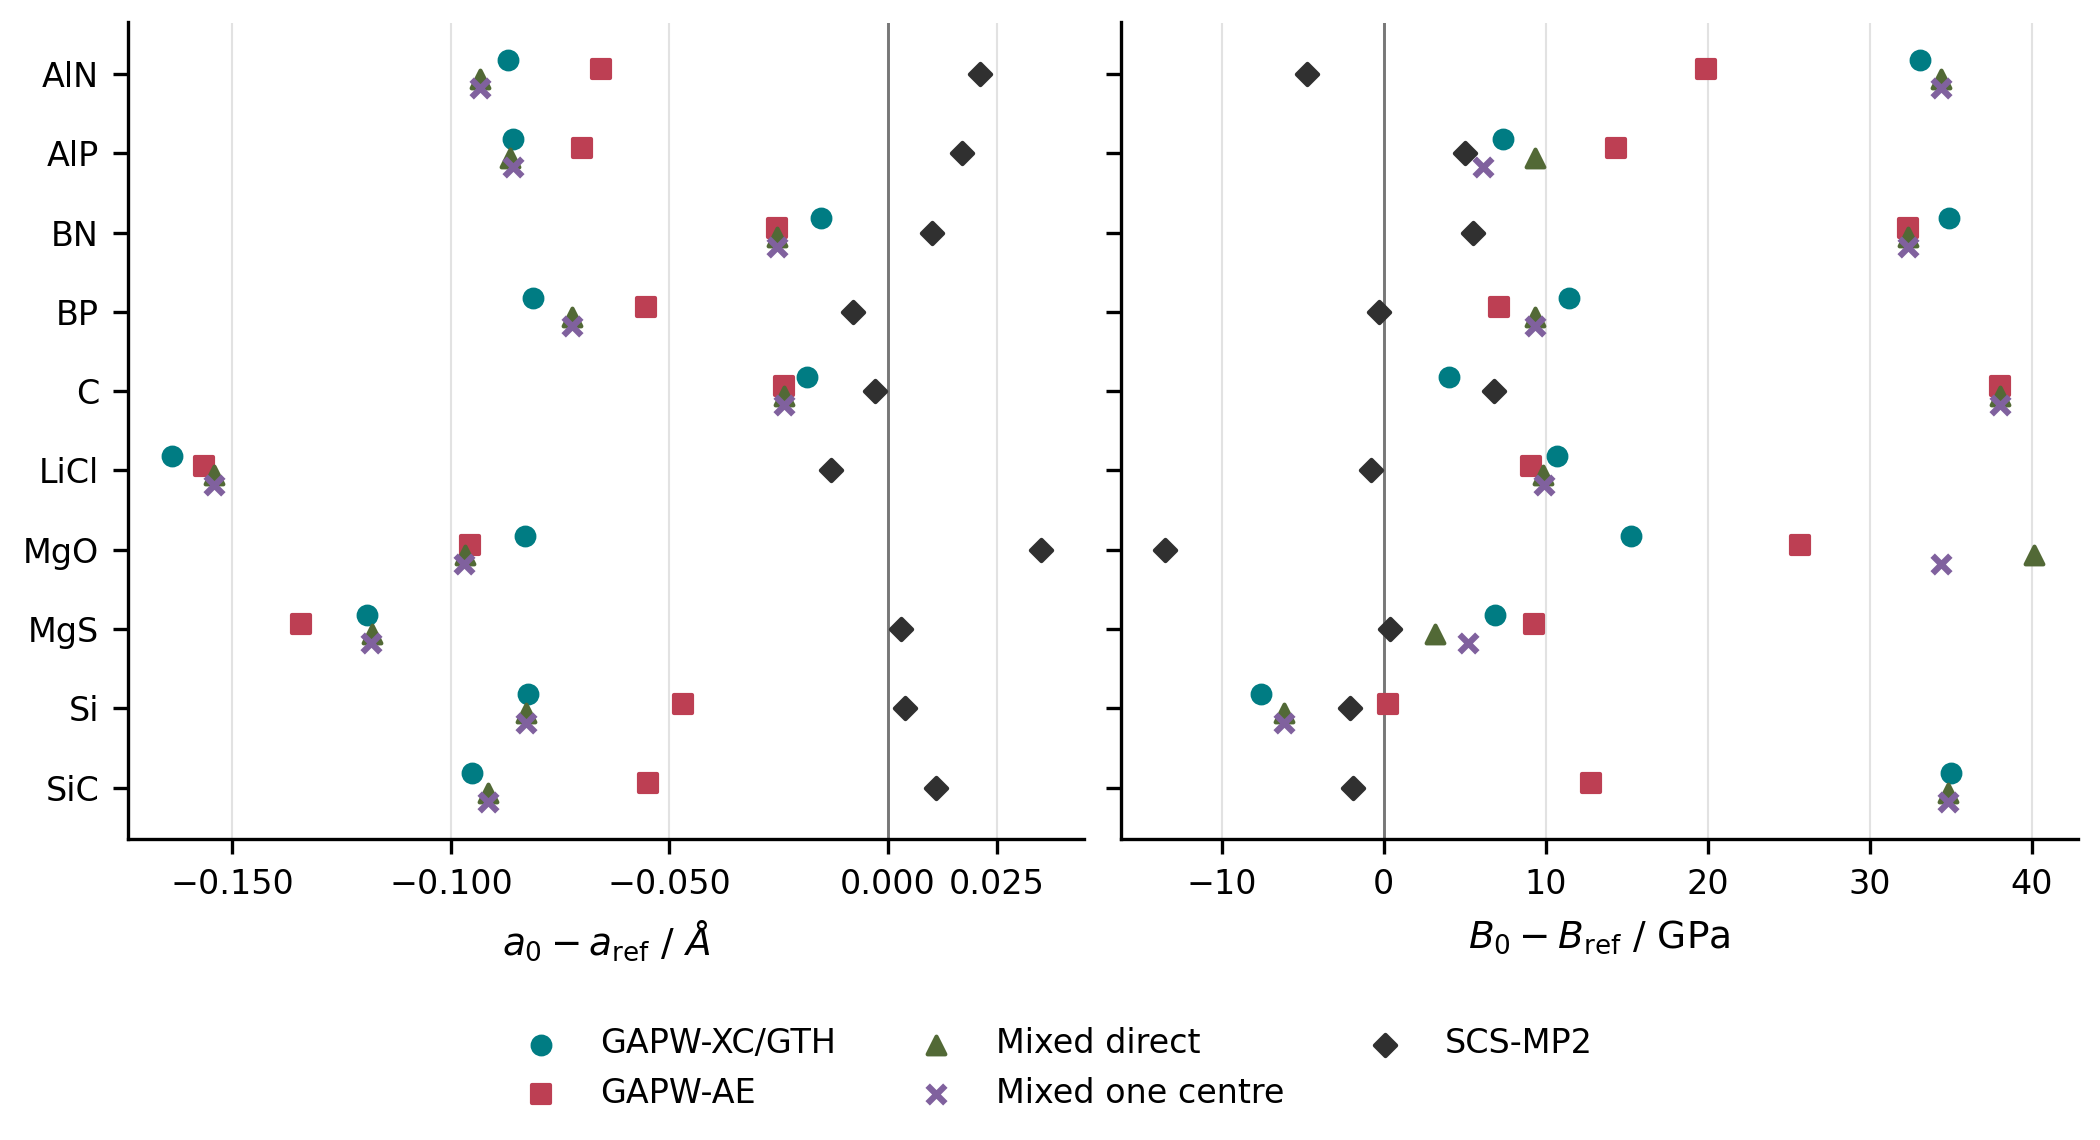
\includegraphics[width=\textwidth]{eos-literature-residuals.png}
\caption{Signed lattice-constant and bulk-modulus errors against the common Goldzak static-lattice reference. SCS-MP2 provides matched correlated-method context. Systematic native lattice contraction persists across representations. Its sign alone does not identify the source of the discrepancy.}
\label{fig:periodic-residuals}
\end{figure}
